\section{Literature Review}

\subsection{Software Quality}
\begin{frame}
\label{subsection:software_quality}
\frametitle{Software Quality}

\begin{definition}
Software quality is the degree to which software possesses a desired combination of attributes (IEEE, 1998). The desired attributes are called \emph{software quality attributes}.
\end{definition} \pause

\begin{example}
\begin{itemize}
  \item Maintainability
  \item Efficiency
  \item Reliability
\end{itemize}
\end{example}

\hyperlink{appendix:software_quality_attributes}{\beamerbutton{More Examples}}

\end{frame}

\subsection{Software Quality Metric}
\begin{frame}
\label{subsection:software_quality_metric}
\frametitle{Software Quality Metric}

We have many software quality metrics.

\begin{example}
\begin{itemize}
  \item Weighted methods per class
  \item Depth of inheritance tree
  \item Coupling factor
\end{itemize}
\end{example}

\hyperlink{appendix:software_quality_metrics}{\beamerbutton{More Examples}}

\end{frame}

\subsection{Goal Question Metric}
\begin{frame}
\label{subsection:goal_question_metric}
\frametitle{Goal Question Metric}

We use Goal Question Metric (GQM) to relate software quality metrics (quanlitative) to software quality attributes (quantitative).

\begin{definition}
Goal Question Metrics is a goal oriented data collection for collecting valid software engineering data. (Basili and Weiss, 1984)
\end{definition} \pause

\begin{example}
\begin{tabular}{ l l }
Goal &: Analysability \\
Question &: Are conditional statements have reasonable depth? \\
Metrics &: Depth of conditional nesting\\
Score &: 90\% (based on benchmark)\\
\end{tabular}
\end{example}

\hyperlink{appendix:goal_question_metric}{\beamerbutton{More Examples}}

\end{frame}

\subsection{Existing Tool: SonarQube}
\begin{frame}[allowframebreaks]
\frametitle{Existing Tool: SonarQube}

\begin{columns}
\column{0.5\textwidth}
SonarQube is a continuous code inspection tool. Features:
\begin{itemize}
  \item Object-oriented metrics
  \item Code style checking
  \item Code duplication detection
  \item Custom configurations for different projects
  \item Support 20 programming languages
\end{itemize}
\column{0.5\textwidth}
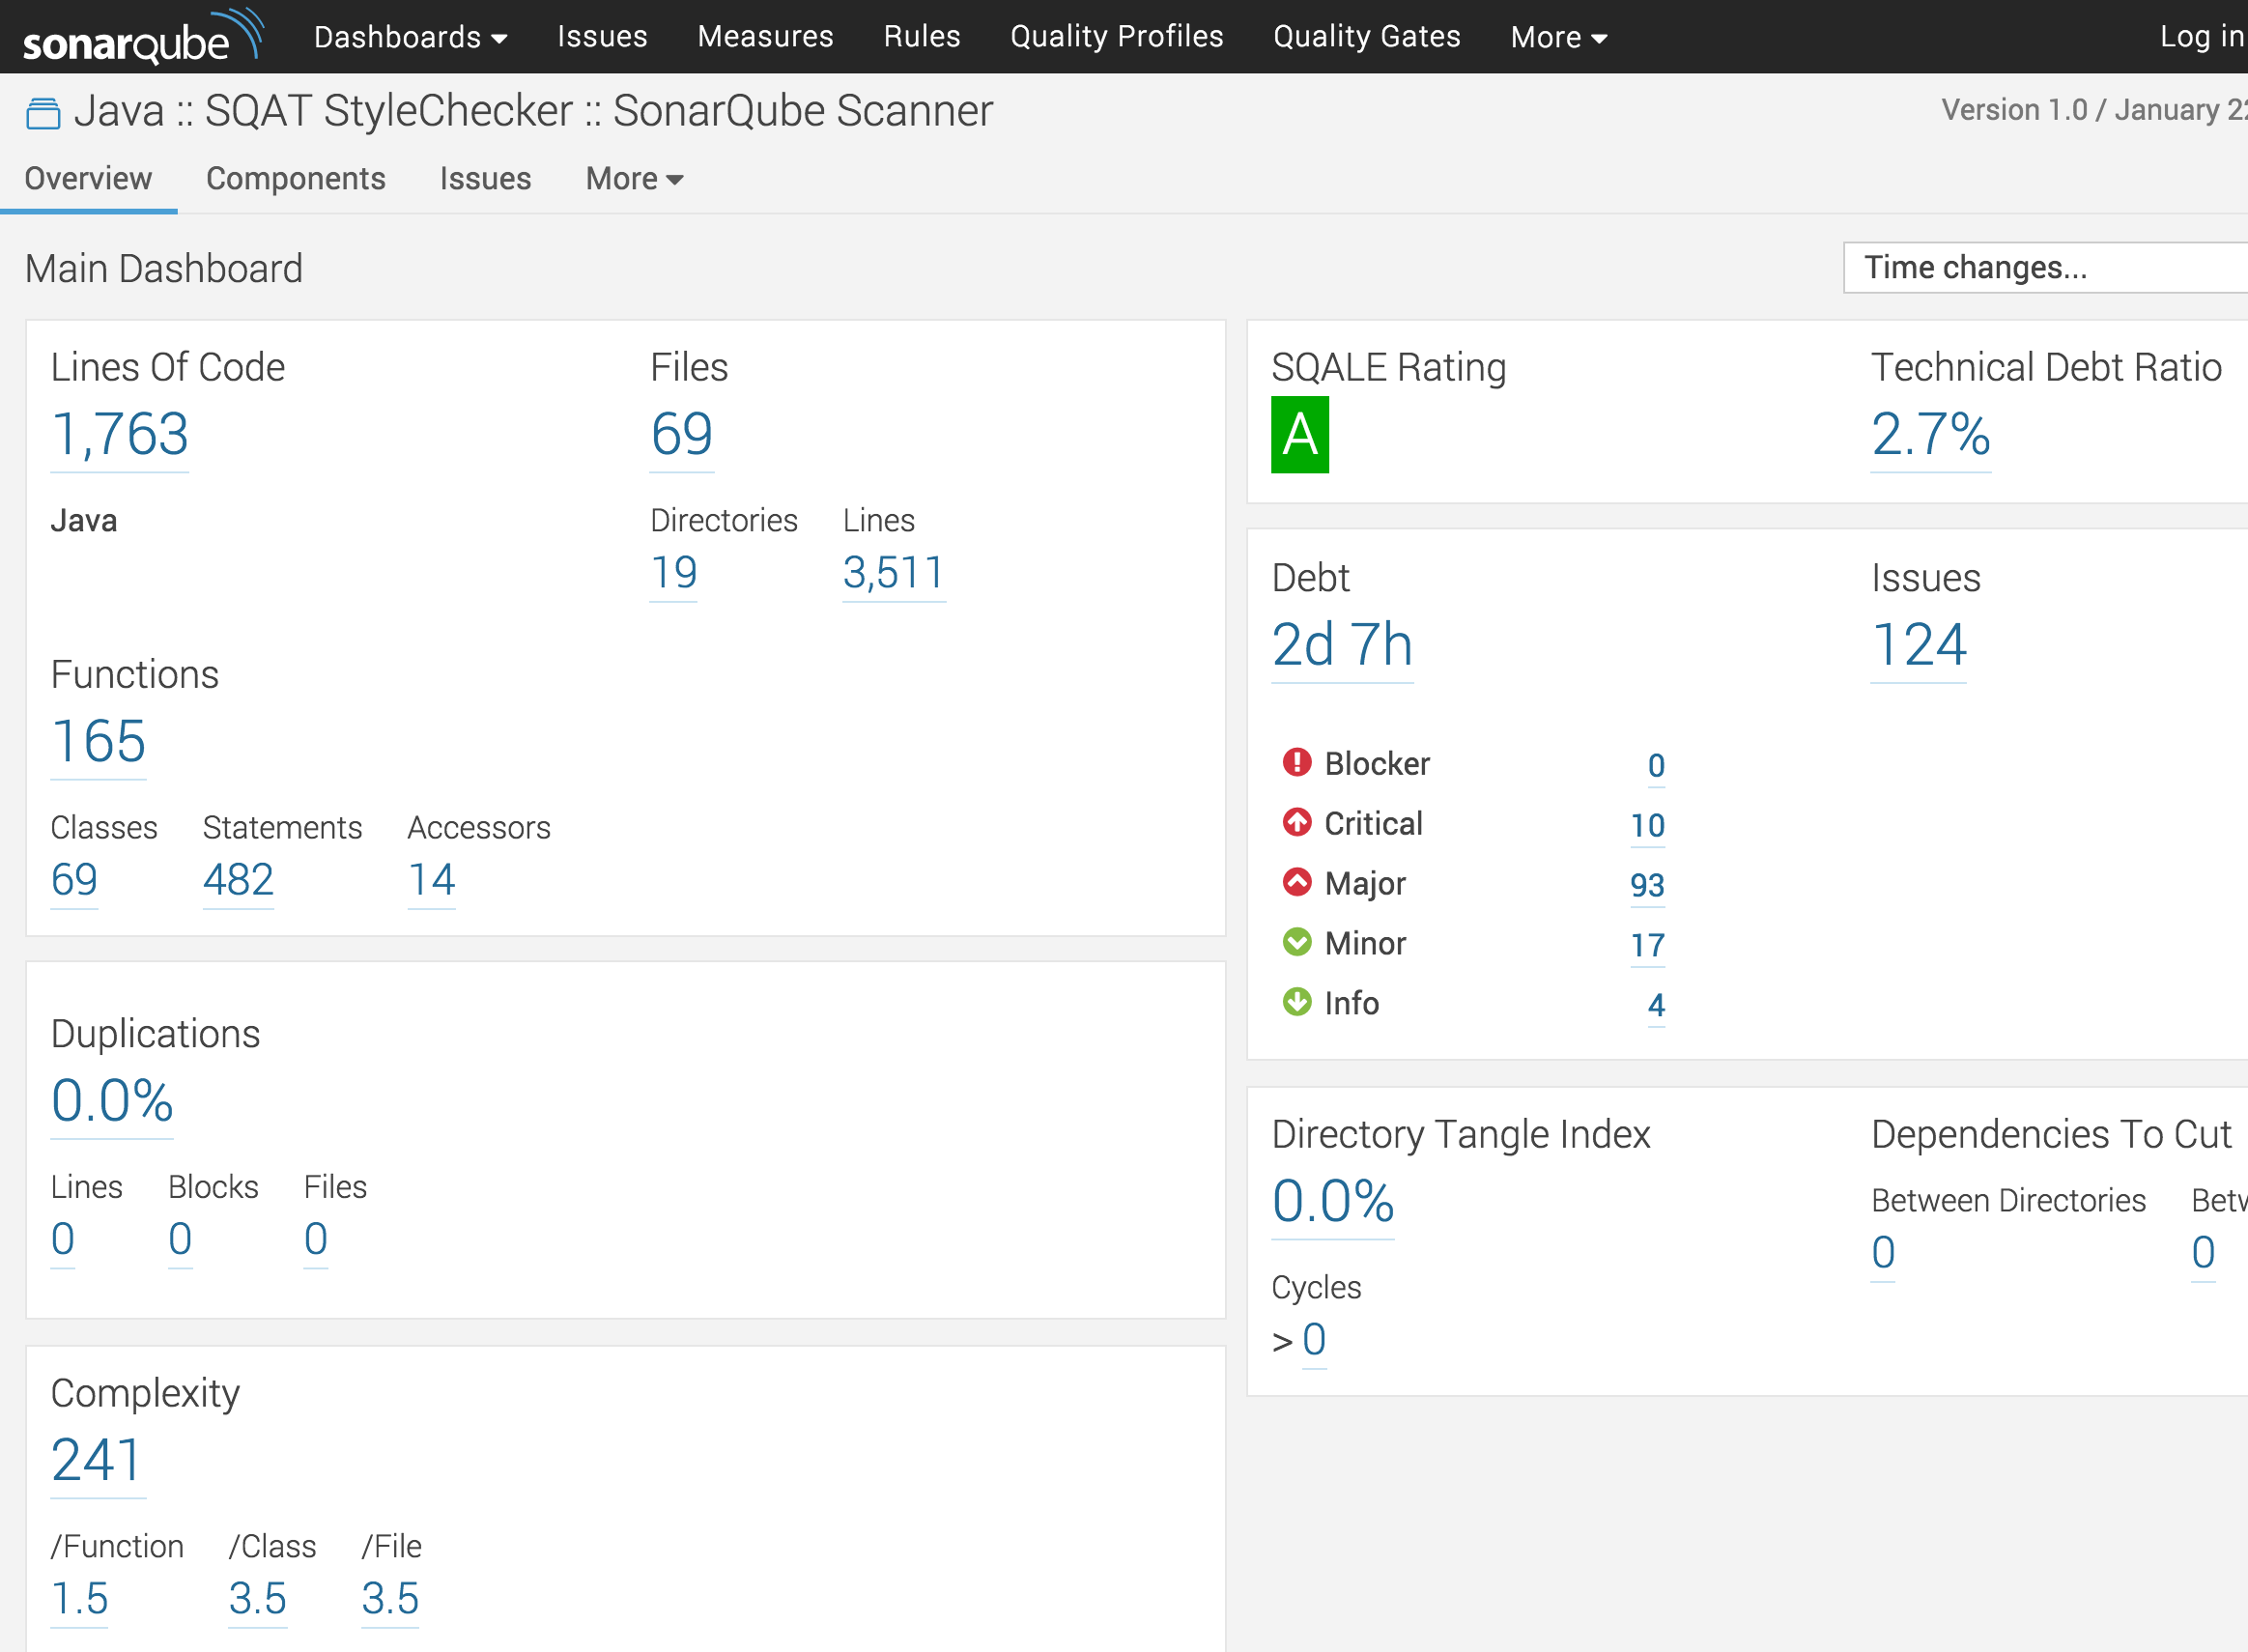
\includegraphics[scale=0.1]{sonar_project_dashboard}
\end{columns}

\framebreak

We do not use SonarQube because:
\begin{itemize}
  \item Need to develop SonarQube plug-in
  \item Do not provide complete API to work with plug-in
    \item Two projects with different goals
  \begin{itemize}
    \item Has user interface for monitoring
    \item Do not have automation tools
  \end{itemize}
\end{itemize}

We decided to develop SQAT from scratch.

\end{frame}